\documentclass{beamer}
\usepackage[utf8]{inputenc}
\usepackage[spanish]{babel}
\usetheme[pageofpages=de,% String used between the current page and the
                         % total page count.
          bullet=circle,% Use circles instead of squares for bullets.
          titleline=true,% Show a line below the frame title.
          alternativetitlepage=true,% Use the fancy title page.
          titlepagelogo=fig/logo,% Logo for the first page.
          %watermark=fig/watermark,% Watermark used in every page.
          %watermarkheight=80px,% Height of the watermark.
          %watermarkheightmult=4,% The watermark image is 4 times bigger
          ]{Torino}
          
\usecolortheme{freewilly}
%\usecolortheme{nouvelle}

\author{Estudiante: {\footnotesize Sebastián Schiavinato} \\ Director: {\footnotesize Dr. Hernán E. Grecco} \\ Codirectora: {\footnotesize Dr. Andrea V. Bragas}}
\title{Determinación de características ópticas del SPIM para la medición de anisotropía de muestras biológicas}
\institute{Laboratorio 6 y 7, DF, FCEyN, UBA}
\date{Julio 5, 2016}

\begin{document}

    \begin{frame}[plain]
        \titlepage
    \end{frame}
    \section{Motivaciones y conceptos}
            En el Laboratorio de Electrónica Cuántica (LEC) se dispone de un microscopio SPIM (de Single Plane Ilumination Microscope, o microscopio de iluminación de plano único). Este microscopio hace uso de muestras con fluoroforos e ilumina en cada instante las muestras con una hoja de laz (lightsheet). Esto elimina el photobleaching, o blanqueo de los flouroforos, y a su vez si se miden varias planos se puede generar una imagen 3D de la muestra.
        
    La construcción de este microscopio requiere determinar
    \begin{itemize}
        \item El perfil del haz a la entrada del microscopio, ya que este haz determina el tamaño de la hoja del haz.
        \item El perfil del haz a la salida del telescopio, antes del objetivo, ya que este debe enfocar en el objetivo para disminuir el tamaño del lightsheet
        \item El espectro del haz, ya que determina los flouroforos a utilizar
        \item Finalmente, la polarización del haz. Si esta polarización es lineal permite hacer mediciones de anisotropía, es decir la distribución en el espacio, de los fluoroforos
    \end{itemize}
            
    Con miras de poder calibrar este microscopio, se diseño y construyó instrumental portátil, que sea de fácil colocación y uso. En particular se construyeron
    \begin{itemize}
        \item Perfilador
        \item Polarimetro
    \end{itemize}




        \begin{frame}[fragile]{Concepto del perfilador}

    \begin{columns}
        \begin{column}{0.5\textwidth}
        
            \begin{itemize}
                \item Perfiladores con cámaras CCD. Sensores muy caros
                \item Perfiladores integradores. Complejidad mecánica
            \end{itemize}
        \end{column}
        
        \begin{column}{0.5\textwidth}
            \begin{figure}[H]
            \centering
            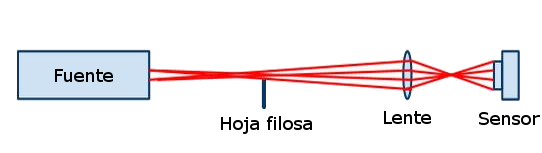
\includegraphics[width=\textwidth]{fig/perfilador/esquema_basico}
            \label{fig:perfilador/esquema_basico}
            \end{figure}
            \begin{figure}
                \centering
                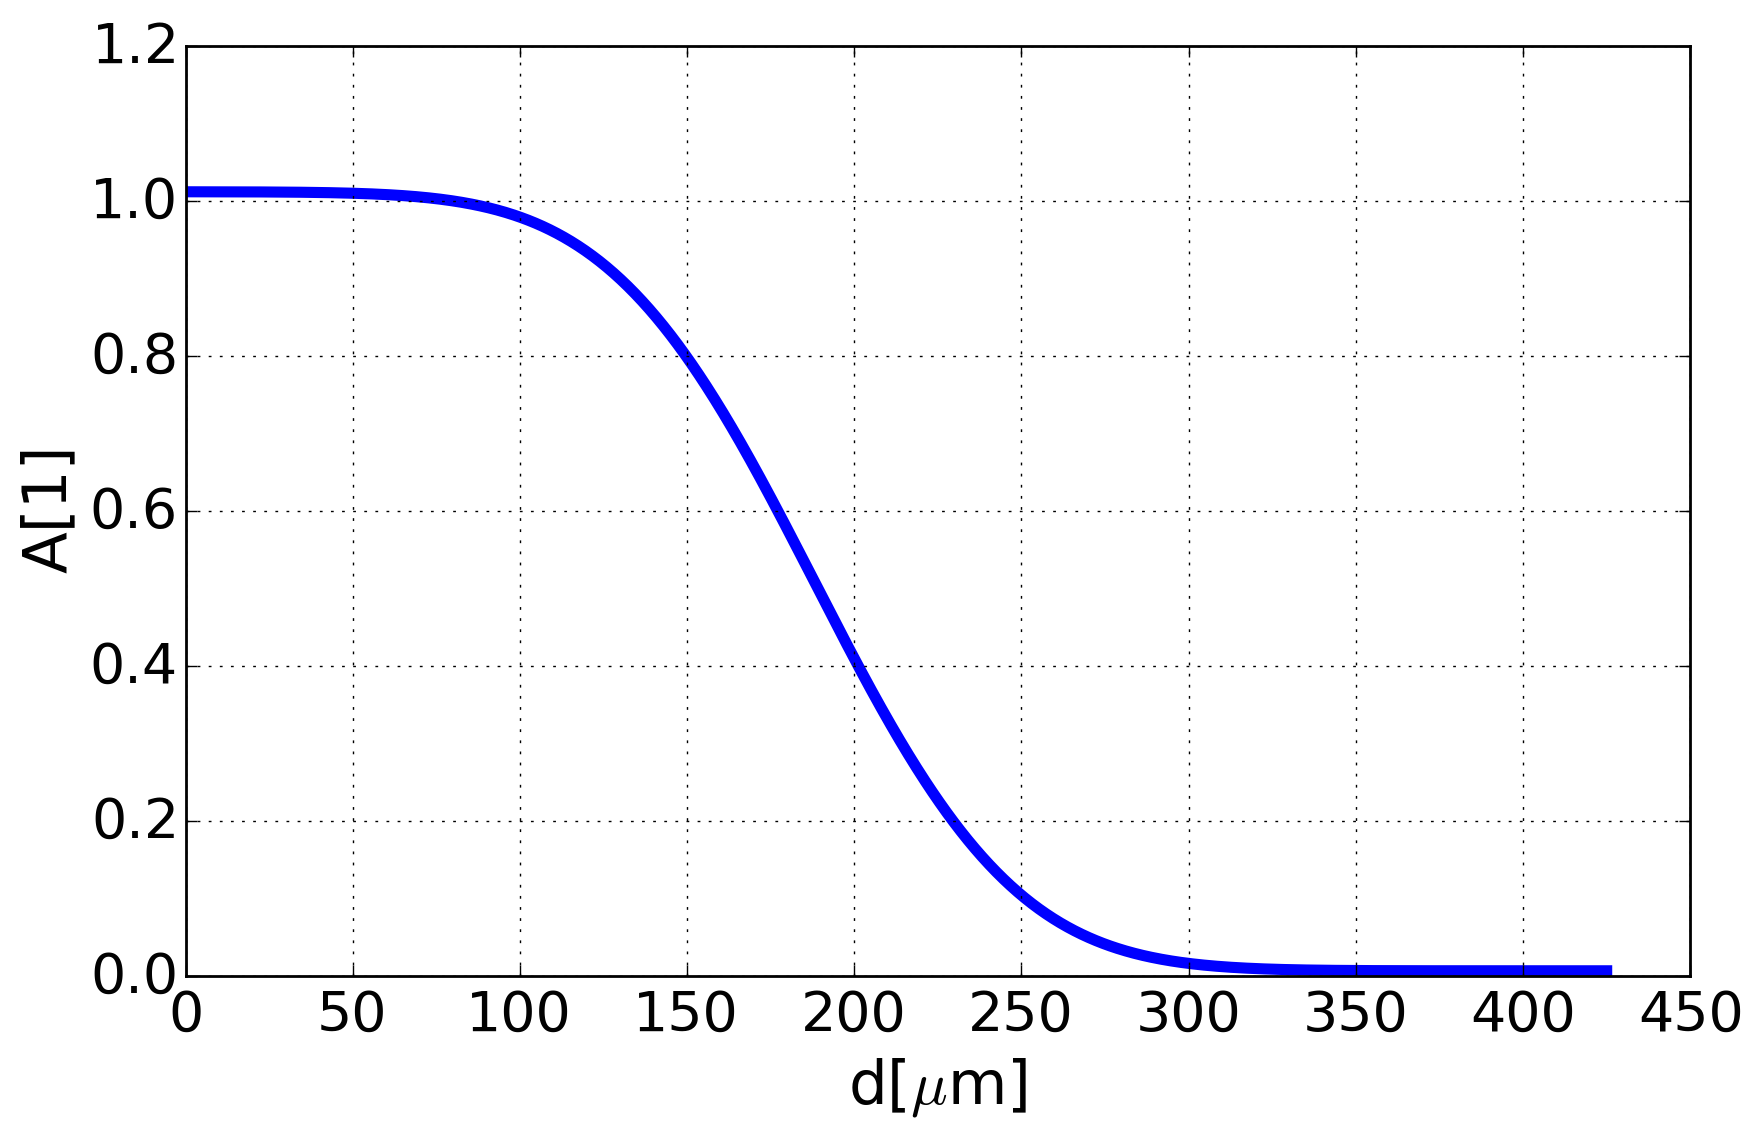
\includegraphics[width=0.8\textwidth]{fig/perfilador/err_function.png}
                \label{fig:perfilador/err_function}
            \end{figure}
        \end{column}
    \end{columns}



\end{frame}

\begin{frame}[fragile]{Concepto del polarizador}
        \begin{figure}[H]
                    \centering
                    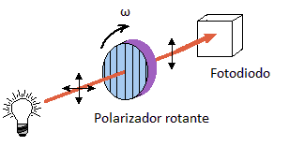
\includegraphics[width=0.5\textwidth]{fig/polarimetro/esquema}
                    %\caption{}
                    \label{fig:polarimetro}
            \end{figure}
        \begin{columns}
            \begin{column}{0.5\textwidth}
                
                \begin{figure}[H]
                    \centering
                    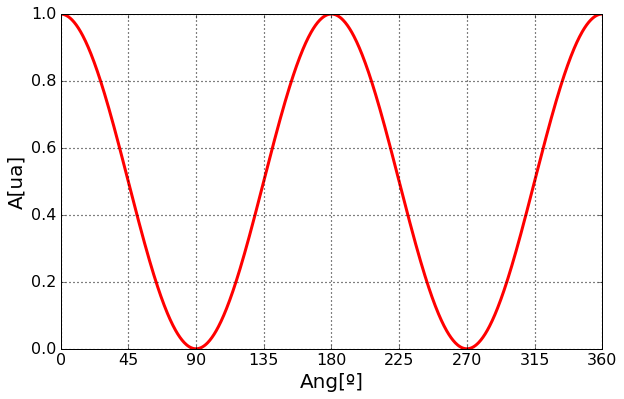
\includegraphics[width=0.7\textwidth]{fig/polarimetro/malus}
                    %\caption{}
                    \label{fig:polarimetro}
                \end{figure}
            \end{column}
            \begin{column}{0.5\textwidth}
                
                \[ \alpha = \frac{\max - \min}{\max + \min} = \begin{cases} 1 & \text{lineal} \\ 0 & \text{circular} \end{cases}\]
            \end{column}
        \end{columns}
   
\end{frame}

    \section{Laboratorio 6}
        \begin{frame}{Resultados prelimiares}

    

    \begin{onlyenv}<1>
        Piezas mecánicas del perfilador
        \begin{columns}[c]
            \begin{column}{.6\textwidth}
                \begin{figure}
                    \centering
                    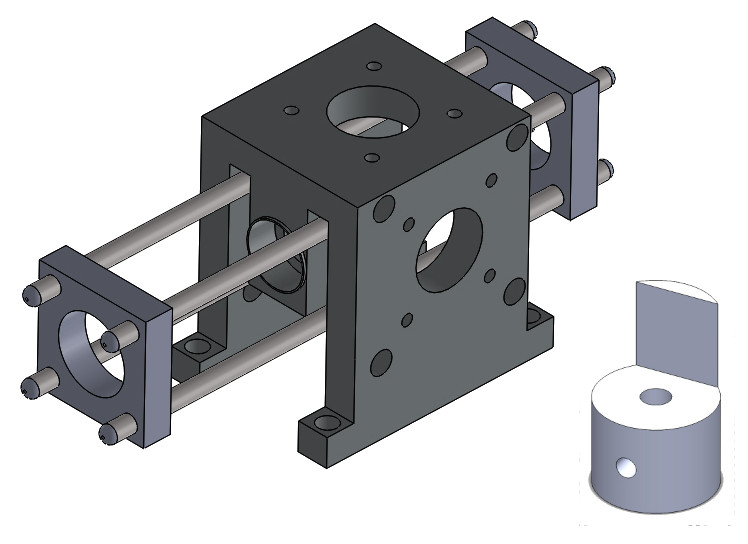
\includegraphics[width=\textwidth]{fig/perfilador/soporte_labo6}
                    \label{fig:pieza}
                \end{figure}
            \end{column}
            \begin{column}{0.4\textwidth}
                \centering
                \begin{figure}
                    \centering
                    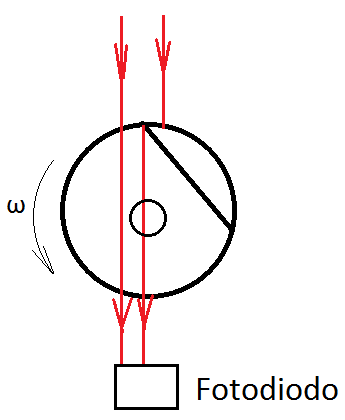
\includegraphics[width=0.8\textwidth]{fig/perfilador/corte_tambor}
                    \label{fig:pieza}
                \end{figure}
                Esquema de la perfilación del tambor
            \end{column}
        \end{columns}
    \end{onlyenv}

    \begin{onlyenv}<2>
        Electrónica de adquisición
        \begin{columns}[c]
            \begin{column}{0.3\textwidth}
                \begin{figure}
                    \centering
                    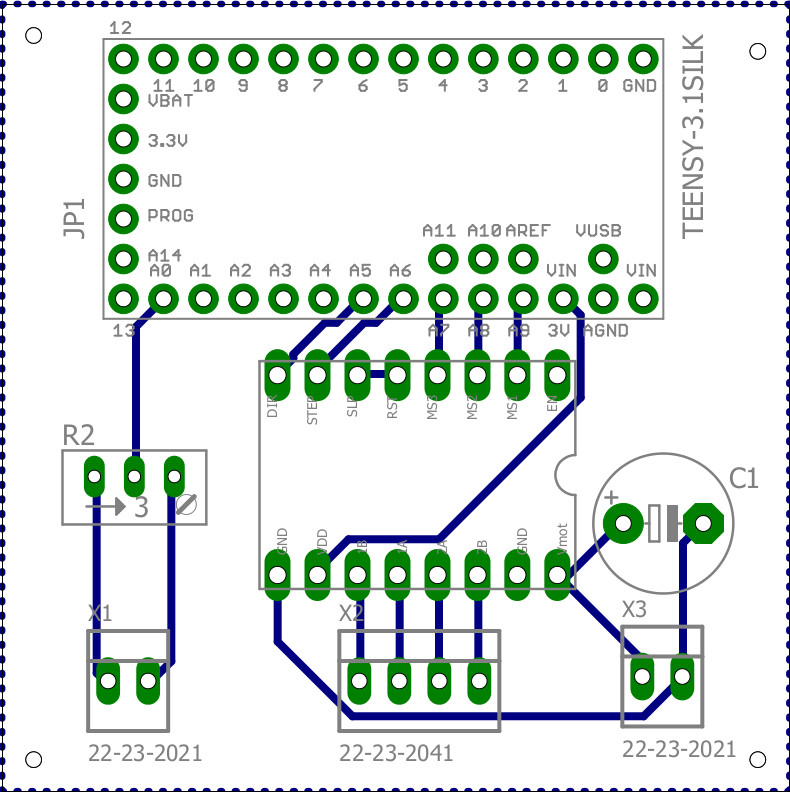
\includegraphics[width=\textwidth]{fig/circuito/circuito_labo6.jpg}
                    \label{fig:circuito}
                \end{figure}
            \end{column}
            \begin{column}{0.6\textwidth}
                \begin{itemize}
                    \item uC Teensy v3.2. CPU 96MHz, y 64KiB RAM. ADC 1Msps max. x10 Arduino Uno
                    \item Placa circuital de 5x5cm. Controla el motor y la adquisición al mismo tiempo. 
                    \item Ajuste de los datos por software. Hecho en Python
                    \item Máxima adquisición de 12 perfiles por segundo, limitación del uC/Software.
                \end{itemize}
            \end{column}
        \end{columns}
    \end{onlyenv}
    \end{frame}
    
    \begin{frame}{Mediciones prelimiares}
        \begin{onlyenv}<1>
        Mediciones a salida de colimador F220FC.
        \begin{columns}[c]
            \begin{column}{0.6\textwidth}
                 \begin{figure}
                    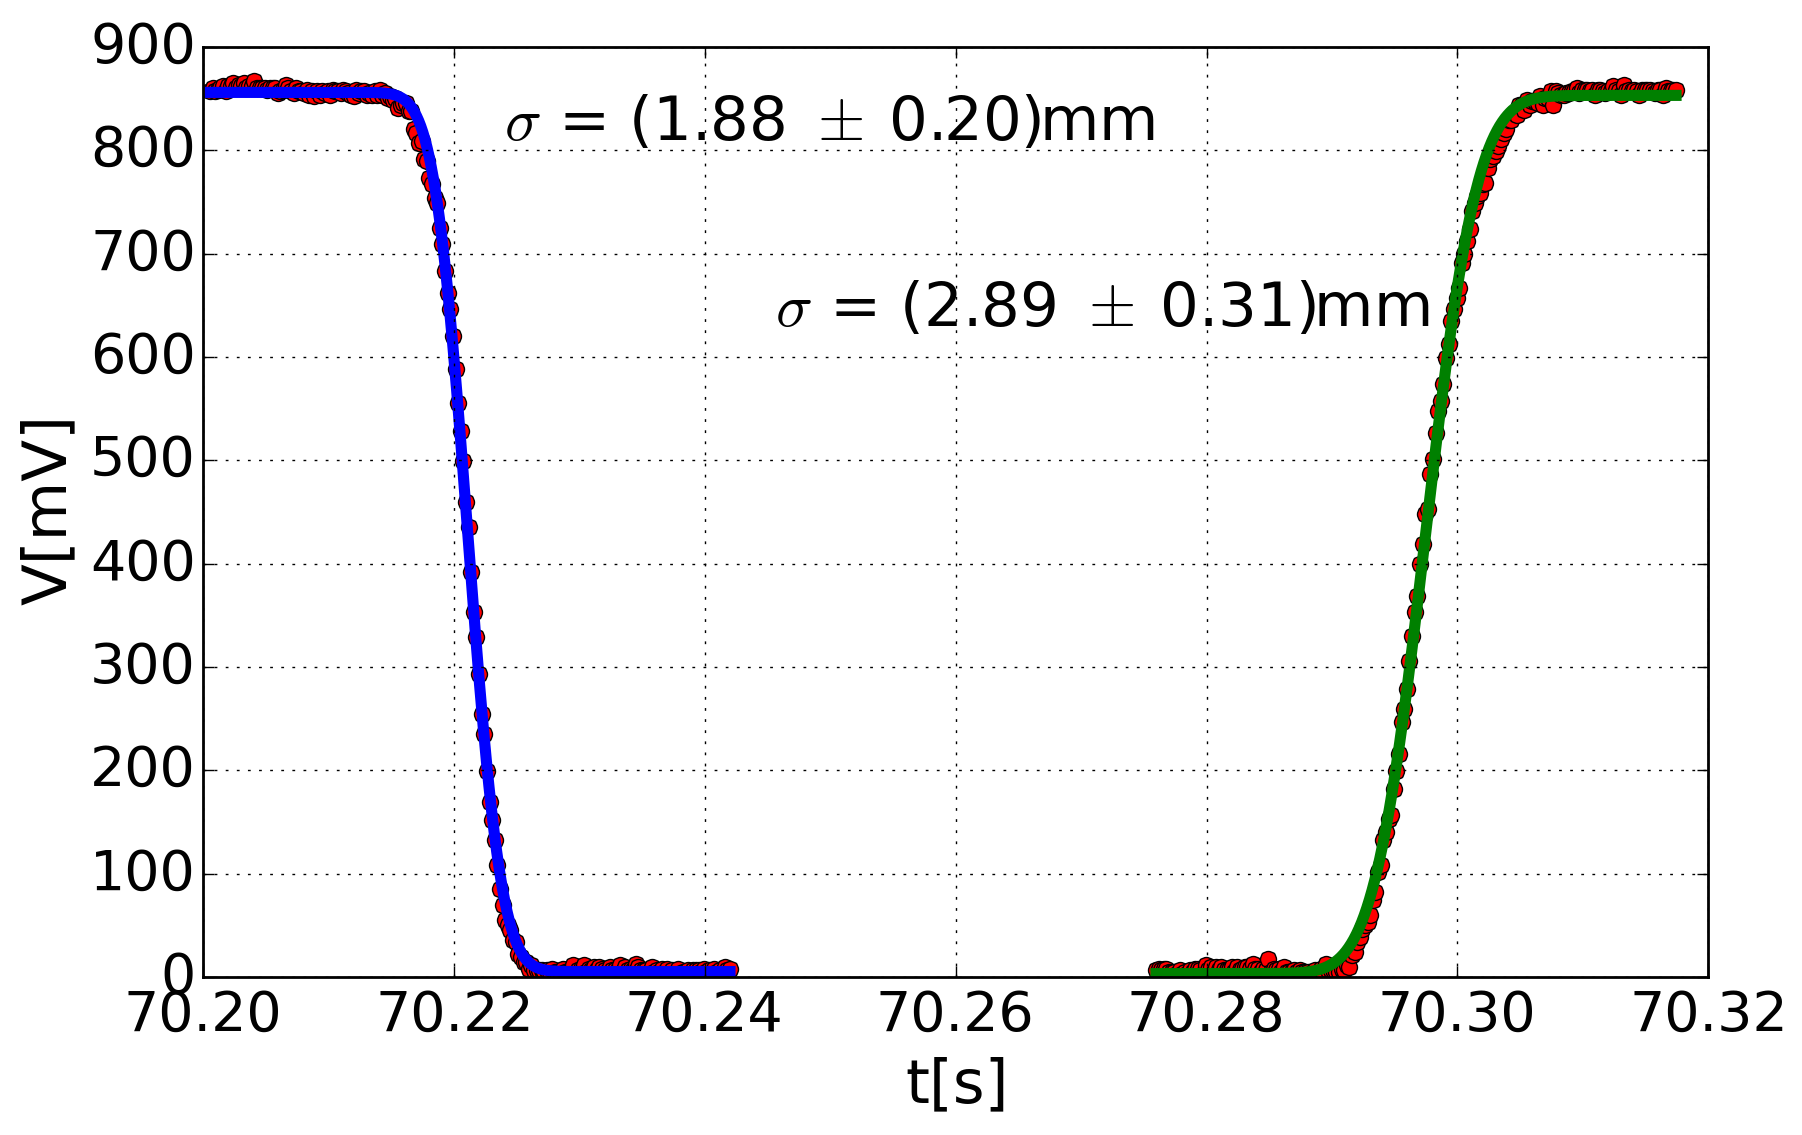
\includegraphics[width=\textwidth]{fig/perfilador/fit_data_labo6}
                    \label{fig:perfilador/fit_data_labo6}
                \end{figure} 
                
               
            \end{column}

            \begin{column}{0.4\textwidth}
                 \begin{figure}
                    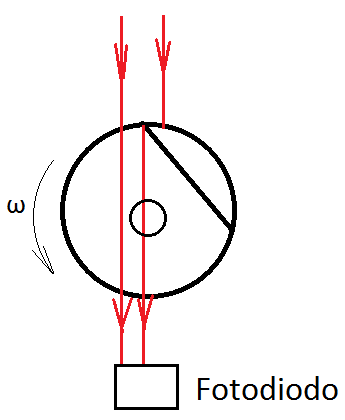
\includegraphics[width=0.4\textwidth]{fig/perfilador/corte_tambor}
                    \label{fig:perfilador/corte_tambor}
                \end{figure} 
                \begin{itemize}
                    \item Diferencia apreciable de tamaño de haz entre transiciones.
                    \item Es de origen mecánico, soporte no ajusta correctamente el motor
                \end{itemize}
            \end{column}
        \end{columns}
        
    \end{onlyenv}
    \begin{onlyenv}<2>
        
        \begin{columns}[c]
            \begin{column}{0.6\textwidth}
                \begin{figure}
                    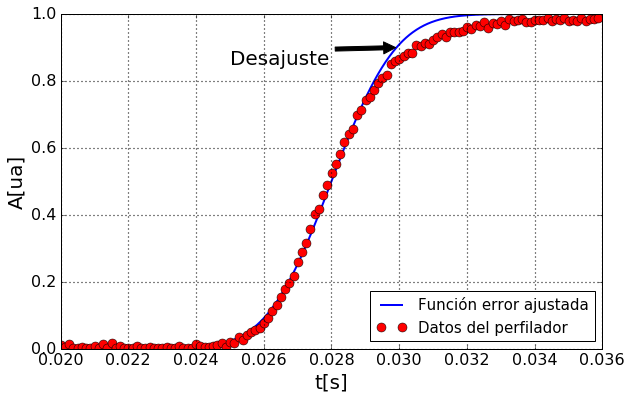
\includegraphics[width=\textwidth]{fig/perfilador/fit_data_labo6_anotado}
                    \label{fig:perfilador/fit_data_labo6_anotado}
                \end{figure} 
             \end{column}

            \begin{column}{0.4\textwidth}
                \begin{itemize}
                    \item Desajuste entre función error y datos al desobturar haz.
                    \item Fotodiodo con resistencia de carga enorme genera respuesta en frecuencia pobre.
                    \item Es necesario amplificar señal del fotodiodo
                \end{itemize}
            \end{column}
        \end{columns}
    \end{onlyenv}
\end{frame}

    \section{Laboratorio 7}
        \subsection{Perfilador}
            
En laboratorio 7, se repensó el perfilador con un soporte con mayor agarre del motor, además de un sistema más simple para colocarlo rápidamente en la mesa óptica. El primer diseño se puede ver en la figura y tiene las siguiente propiedades
\begin{itemize}
    \item Soporte adosable a la mesa óptica por perros. Facil colocación
    \item Motor encastrado en soporte. No hay artefactos mecánicos
    \item Tambor de metal con superficie no reflectante
    \item No permite medir fácilmente en el otro eje. Habrá otra iteración
\end{itemize}
    
Posteriormente, se utilizó un motor más pequeño, un NEMA 8, para achicar aún más el diseño (unas 5 veces). De esta forma este soporte permite utilizarse fácilmente en ambos ejes, y no solo eso, se encontró que el tambor de plástico funciona correctamente para perfilar la señal.


        \subsection{Polarímetro}
            \begin{frame}{Mecánica del polarimetro}
    \begin{columns}
        \begin{column}{0.5\textwidth}
            \begin{figure}[H]
                \centering
                
\includegraphics[width=0.8\textwidth]{fig/polarimetro/soporte_all}
                \label{fig:polarimetro/soporte_all}
            \end{figure}
        \end{column}
        \begin{column}{0.5\textwidth}
            \begin{itemize}
                \item Motor NEMA 8 mueve el engranaje inferior paso a paso
                \item Utiliza electrónica creada para el perfilador. Mide en cada paso del motor
                \item Hecho con impresión 3D en plástico
            \end{itemize} 
        \end{column}
    \end{columns}
\end{frame}

        \subsection{Electrónica de adquisición}
            
\begin{frame}{Electrónica de adquisición}
\begin{columns}[c]
    \begin{column}{0.4\textwidth}
        \begin{itemize}
        \item Implementado amplificador de transimpedancia con fotodiodo no polarizado. 
        \item Mejor respuesta en frecuencia y ajusta correctamente una función error.
        \end{itemize}
    \end{column}
    \begin{column}{0.6\textwidth}
        
        \vspace{-1em}
        \begin{figure}[H]
            \centering
            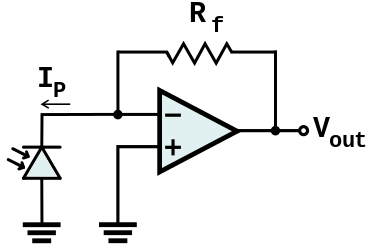
\includegraphics[width=0.5\textwidth]{fig/circuito/amp/TIA.png}
            \label{fig:circuito/amp/TIA}
        \end{figure}
        \vspace{-1em}
         \begin{figure}[H]
                %\centering
                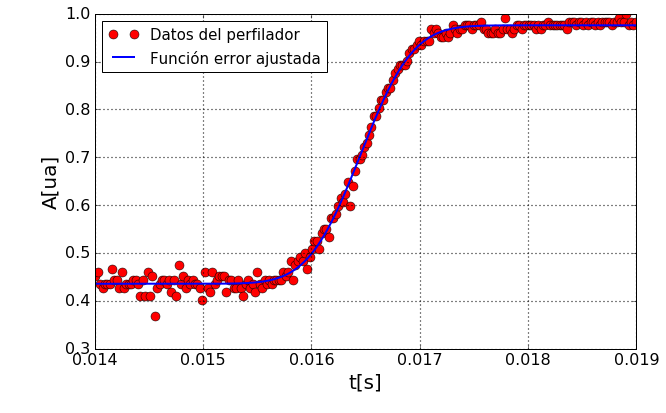
\includegraphics[width=\textwidth]{fig/perfilador/fit_data_plastico_subida.png}
                \label{fig:perfilador/amplificacion_funcional}
        \end{figure}
    \end{column}
\end{columns}



\end{frame}

\begin{frame}{Calibración de amplificador}

\begin{columns}[c]
    \begin{column}{0.4\textwidth}
        \begin{itemize}
        \item Amplificador con LM358. Con fuente simple
        \item Respuesta al escalón de 0,4V$\,\mu$s$^{-1}$. 4 veces más grande de la necesaria
        \item Rango lineal bastante amplio, no marca corriente nula
        \end{itemize}
    \end{column}
    %
    \begin{column}{0.5\textwidth}
        \vspace{-1em}
        \begin{figure}[H]
            \centering
            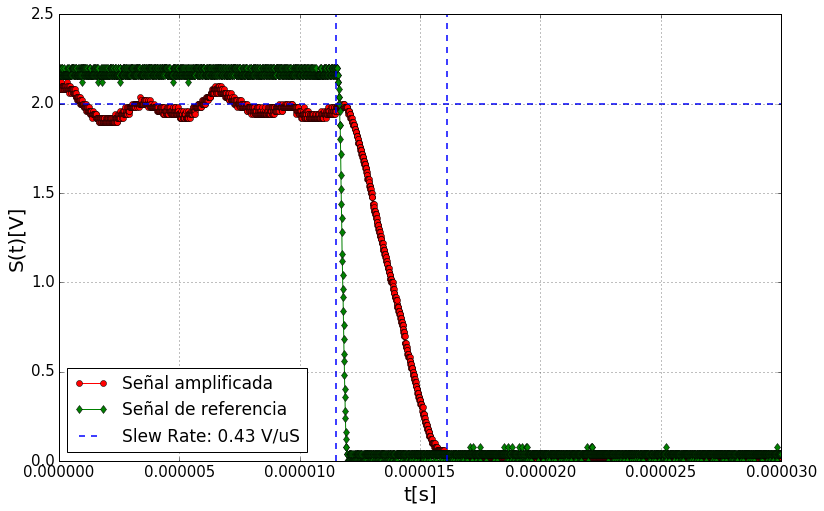
\includegraphics[width=\textwidth]{fig/circuito/amp/transicion_amp}
            \label{fig:transicion_amp}
        \end{figure}
        \vspace{-2em}
        \begin{figure}[H]
            \centering
            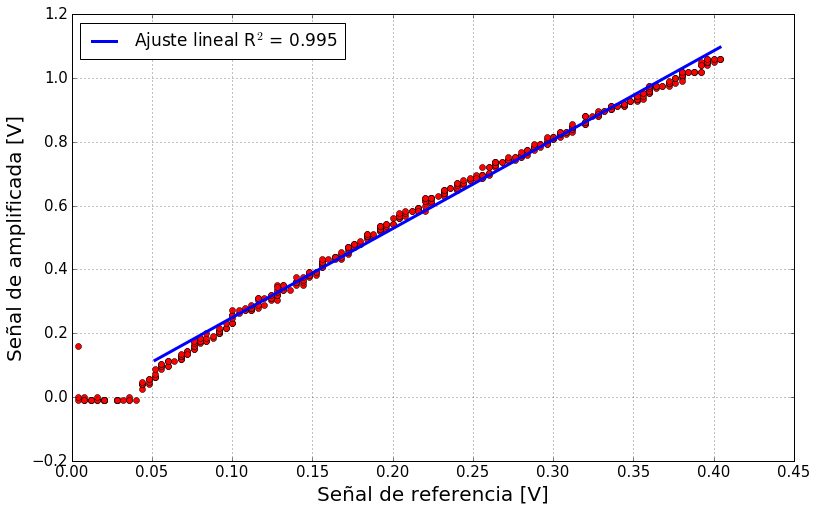
\includegraphics[width=\textwidth]{fig/circuito/amp/lin_amp}
            \label{fig:circuito/amp/lin_amp}
        \end{figure}
    \end{column}
\end{columns}


\end{frame}

\begin{frame}{Generación de sensores portátiles}
    \begin{onlyenv}<1>
        \begin{columns}[c]
            \begin{column}{.5\textwidth}
            Particle.io Photon
            \begin{itemize}
                \item ARM Cortex M3 120MHz, 128KiB RAM y 1MiB Flash, con stack WiFi. x1.5 Teensy
                \item Programación en la nube en C++, permite actualizaciones OTA.
                \item API de programación mejor desarrollada, libre.
            \end{itemize}
            \end{column}

            \begin{column}{.5\textwidth}
                \vspace{-2em}
                \begin{figure}
                    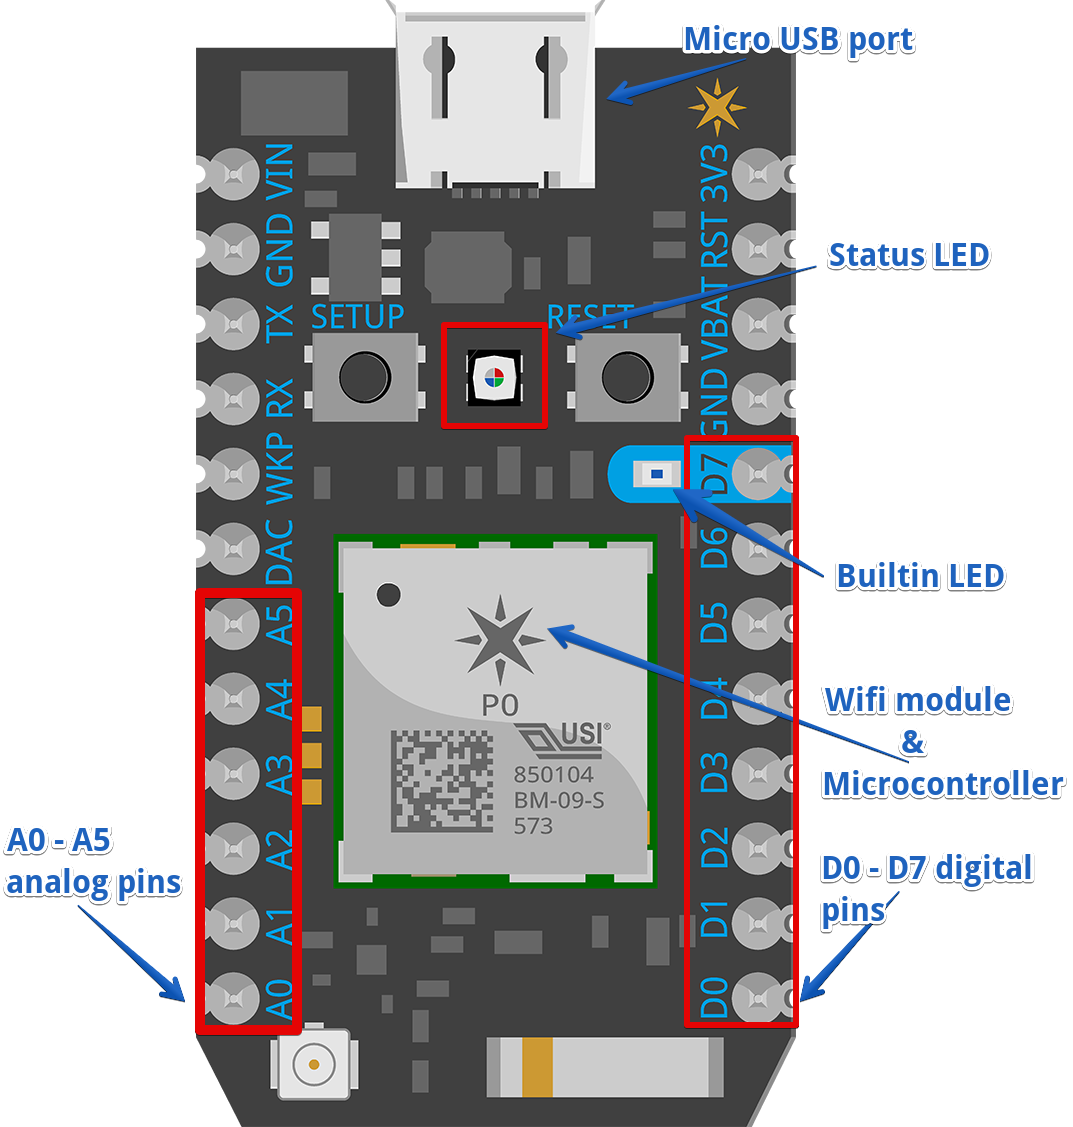
\includegraphics[width=0.8\textwidth]{fig/circuito/photon}
                    \label{fig:circuito/photon}
                \end{figure}
                
            \end{column}
        \end{columns}
    \end{onlyenv}

    \begin{onlyenv}<2>
        \begin{columns}
            \begin{column}{0.7\textwidth}
                \begin{block}{Resultados con este uC/Software}
                    \begin{itemize}
                        \item Se pudo mover el motor hasta 30RPS. \\PWM mejor implementado
                        \item Adquisición de datos (del uC) cada 10$\mu$s o 100ksps. Más de lo necesario
                        \item Conexión TCP ya resuelta, cada 0,1s se obtiene 4000 datos. 
                        \item Software de adquisición hecho enteramente en Python, libre, con interfaz de usuario gráfica
                    \end{itemize}
                \end{block}
            \end{column}
            \begin{column}{0.3\textwidth}
                \begin{figure}
                    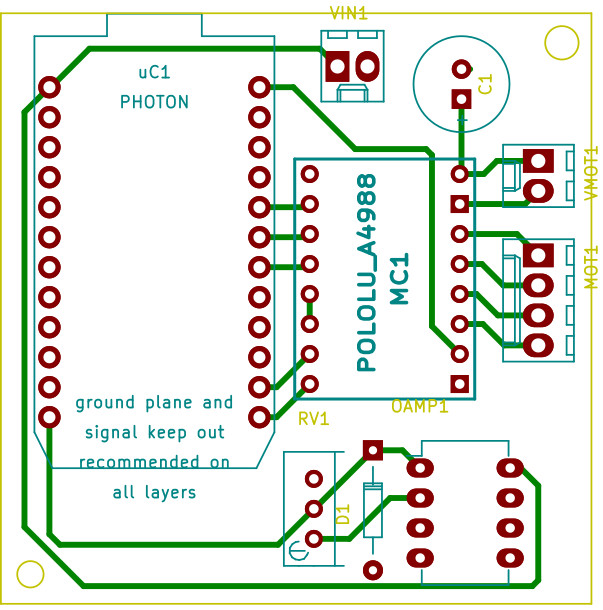
\includegraphics[width=\textwidth]{fig/circuito/circuito_labo7_color}
                    \label{fig:circuito/circuito_labo7_color}
                \end{figure}
            \end{column}
        \end{columns}
    \end{onlyenv}

\end{frame}



    \section{Mediciones}
        \subsubsection{Mediciones con el perfilador}

        Calibración del instrumento, medición del colimador F280FC del SPIM. Se midió al inicio y al final del riel, para observar divergencias
        \begin{itemize}
                \item Inicio del riel:\\ $\sigma = (3,03 \pm 0,15)\,\text{mm}$
                \item Fin del riel:\\ $\sigma = (3,02 \pm 0,18)\,\text{mm}$
        \end{itemize}
        Colimador \underline{efectivamente colima el haz}.
        
        Luego se midicó de forma manual el haz, por medio de una hoja filosa y un tornillo microméticro, y se obtuvo lo que se ve en la figura. 
        
        De esta forma se puede aceverar que el perfilador tiene la misma precisión que el método manual, de alrededor de un 5\%, y además el sistema es exacto en su medición.
            
       
       Finalmente se hizo una medición extra en el telescopio del SPIM para poder observar la divergencia del haz. En la figura se puede observar una diferencia apreciable entre de diferente plano de obturación, lo que demuestra que a divergencia del haz es medible. 
       
       Nos queda poder utilizar el perfilador para determinar las propiedades de la lente cilindrica del SPIM.
 

\subsection{Mediciones con el polarimetro}
        Para poder medir con el polarimetro, primero es necesario calibrar el materia polarizador. Para eso se construyó dos láminas rotantes y se midió la intensidad de un haz linealmente polarizado atravezando ambas láminas alineadas (en el máximo y minimo de intensidad).
         Se encontró que la matriz de transmisión es la siguiente
            \begin{equation*}
                \begin{pmatrix} 0,5 & 0 \\ 0 & 2\times 10^{-6} \end{pmatrix}
            \end{equation*}
            hecho que marca al material polarizador lejos del ideal, ya que elimina el 50\% de la señal en el máximo y no elimina toda la polarización del haz, pero suficiente para hacer una medición cualitativa de la polarización. Para mejorar el sistema se debe utilizar un polarizador con mejores parámetros.
            
            
        Finalmente, se midió la polarización del laser más utilizado en el SPIM, modelo DHOM-M-473-150mW (que es azul en $\lambda = 473$nm), sacando un reflejo del haz antes de la fibra y el haz después de la fibra. Además se agrega el resultado del cociente para determinar la \emph{calidad de polarización lineal}. 
        
        Como se ve la polarización es casi lineal en ambos casos, pero lo más importante es que polarización se mantienen. Este análisis se hizo para varias potencias del haz, pero lamentablemente el polarizador deja de funcionar correctamente. 
        
        El setup también dispone de un láser rojo y un laser verde. El laser rojo se encontró que no mantiene polarización, ya que antes de la fibra el cociente es de $(0,94pm0,32)$ y $(0,39\pm 0,15)$, pero se volverán a medir, pero el laser verde tiene fluctuaciones de potencia por lo que no es muy útil para esta medición.
        

    \section{Conclusiones}
        \begin{frame}{Conclusiones}
    \begin{onlyenv}<1>
    Del polarizador
        \begin{itemize}
            \item El perfilador mide exitosamente el haz, con un error del \%5, comparable con la medición manual 
            \item Se pudo caracterizar el haz a salir de la fibra y en el telescopio correctamente
            \item El perfilador fue capaz de medir la divergencia \underline{con solo un set de mediciones}.
            \item Para medir la salida del telescopio habrá que diseñar un perfilador más compacto.
        \end{itemize}
    \end{onlyenv}
    
    \begin{onlyenv}<2>
        Del polarimetro
        \begin{itemize}
            \item La lámina polarizadora utilizada está lejos de ser un polarizador perfecto, pero es funcional a la aplicación
            \item Se midió la polarización antes de acoplar en fibra y después de acoplar en fibra y \underline{no se observó cambio de polarización}
            \item Esta medición es de importancia fundamental para medir anisotropía de flouroforos en el SPIM
        \end{itemize}
    \end{onlyenv}
\end{frame}

        
    \section{Proyecto SOMA}
        \begin{frame}{Proyecto SOMA (Sistema de OptoMecánica Abierta)}
            \centering
            \begin{figure}[H]
                \centering
                
\includegraphics[width=0.4\textwidth]{fig/proyecto_soma}
                \label{fig:soma}
            \end{figure}
            \begin{itemize}
                \item Plataforma abierta de instrumental opto-mecánico
                \item Diseño con énfasis en la reproducibilidad, con tecnología de impresora 3D o mecanizado automático.
                \item Electrónica libre, controlada por software creado con tecnologías libres.
            \end{itemize}
            Página del proyecto: \url{http://lec.df.uba.ar/soma}
        \end{frame}

        \begin{frame}[plain]{}
            \centering
            \Huge
            Gracias
        \end{frame}
\end{document}

